\documentclass[dvipdfmx,8pt]{beamer}


\usepackage{here, amsmath, latexsym, amssymb, bm, ascmac, mathtools, multicol, tcolorbox, subfig, color, ulem, tikz, graphics, braket,url}
\usepackage{pxjahyper}%しおりの文字化けを防ぐ
\renewcommand{\baselinestretch}{1.2}
\renewcommand{\figurename}{図}
\renewcommand{\tablename}{表}
\renewcommand{\kanjifamilydefault}{\gtdefault}
\usefonttheme{professionalfonts}
\setbeamertemplate{navigation symbols}{}
\AtBeginSection[]{
\frame{\tableofcontents[currentsection, 
hideallsubsections]} %目次スライド
} % セクション毎に目次スライドを入れる

\usetheme{Rochester}

\title{修論ゼミ}
\author[須賀]{須賀勇貴}
\institute[茨大]{茨城大学大学院 \ 理工学研究科 \ 量子線科学専攻 \ 2年}
\date{2023年7月20日}

\begin{document}
\maketitle
\frame{\tableofcontents[hideallsubsections]}

\section{4.2 \ $WW^{\top}$におけるスピン相関}
\begin{frame}[t]{4.2 \ $WW^{\top}$におけるスピン相関}
  \begin{figure}
    \begin{center}
      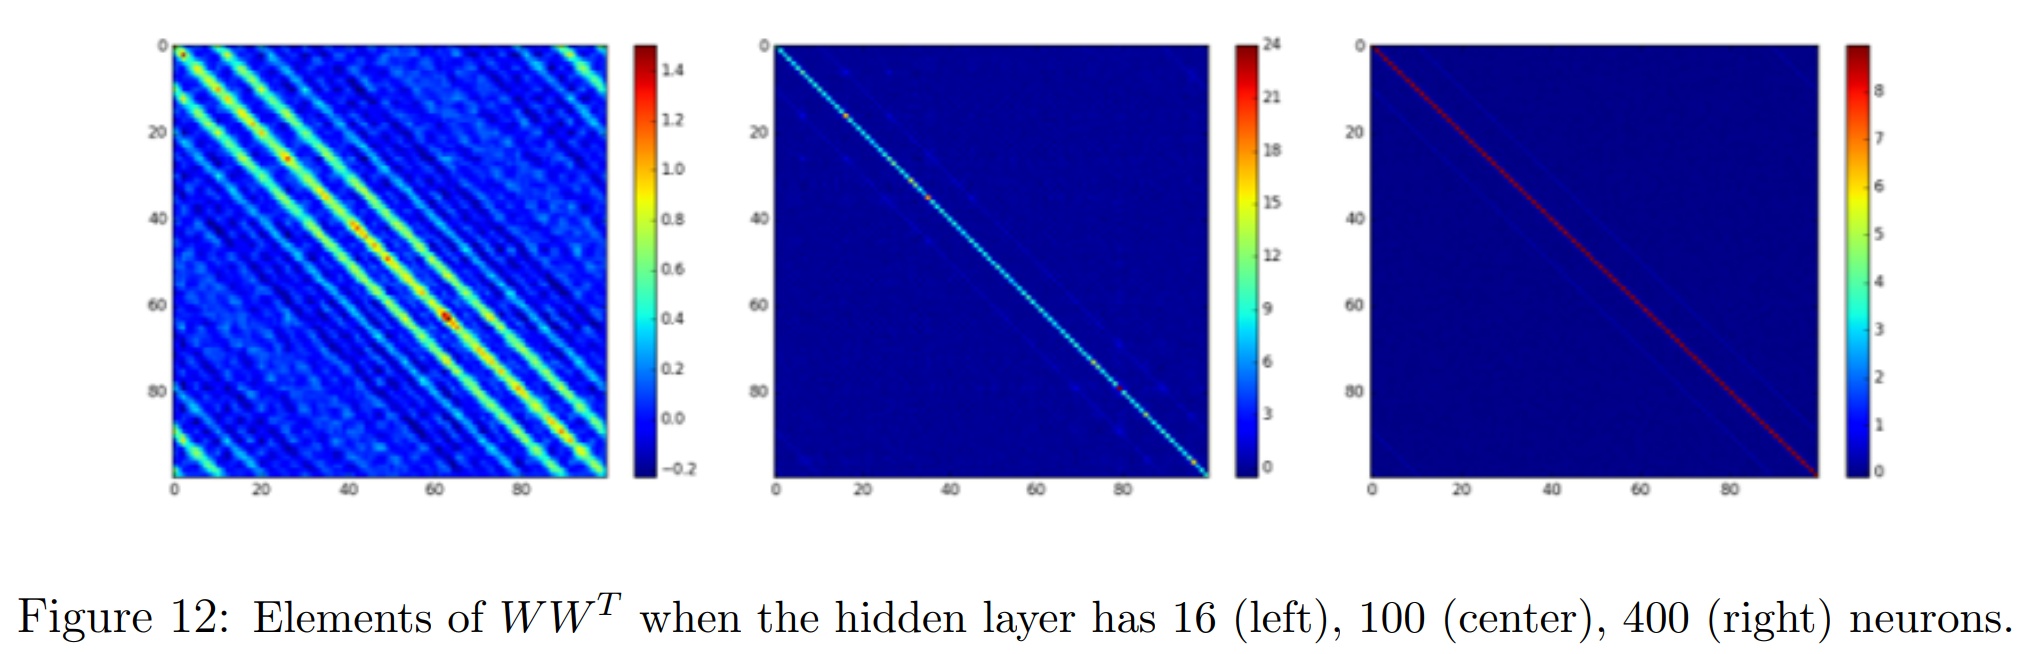
\includegraphics[height=3.6cm]{image/Figure12.png}
    \end{center}
  \end{figure}
  図12はTypeVのRBMでの行列$WW^{\top} \ (100 \times 100)$の各要素の値をプロットしたもの
  \begin{columns}
    \begin{column}{0.7\textwidth}
      \begin{equation*}
        (\sigma_{1,1},\sigma_{1,2},\cdots,\sigma_{1,L},\sigma_{2,1},\cdots,\sigma_{2,L},\sigma_{3,1},\cdots,\sigma_{L,L})
      \end{equation*}
      \begin{equation*}
        \Downarrow
      \end{equation*}
      \begin{equation*}
        (\sigma_1,\sigma_2,\cdots,\sigma_L,\sigma_{L+1},\cdots,\sigma_{2L},\sigma_{2L+1},\cdots,\sigma_{LL})
      \end{equation*}
    \end{column}
    \begin{column}{0.3\textwidth}
      \begin{tikzpicture}
        \draw[dashed](-1,0)--(1,0);
        \draw[dashed](0,-1)--(0,1);
        \draw(0,0)node[below right]{$\sigma_i$};
        \draw(-1,0)node[left]{$\sigma_{i-1}$};
        \draw(1,0)node[right]{$\sigma_{i+1}$};
        \draw(0,-1)node[below]{$\sigma_{i+L}$};
        \draw(0,1)node[above]{$\sigma_{i-L}$};
        \fill(0,0)circle(0.05);
        \fill(-1,0)circle(0.05);
        \fill(1,0)circle(0.05);
        \fill(0,-1)circle(0.05);
        \fill(0,1)circle(0.05);
      \end{tikzpicture}
    \end{column}
  \end{columns}
\end{frame}

\begin{frame}[t]{4.2 \ $WW^{\top}$におけるスピン相関}
  \begin{figure}
    \begin{center}
      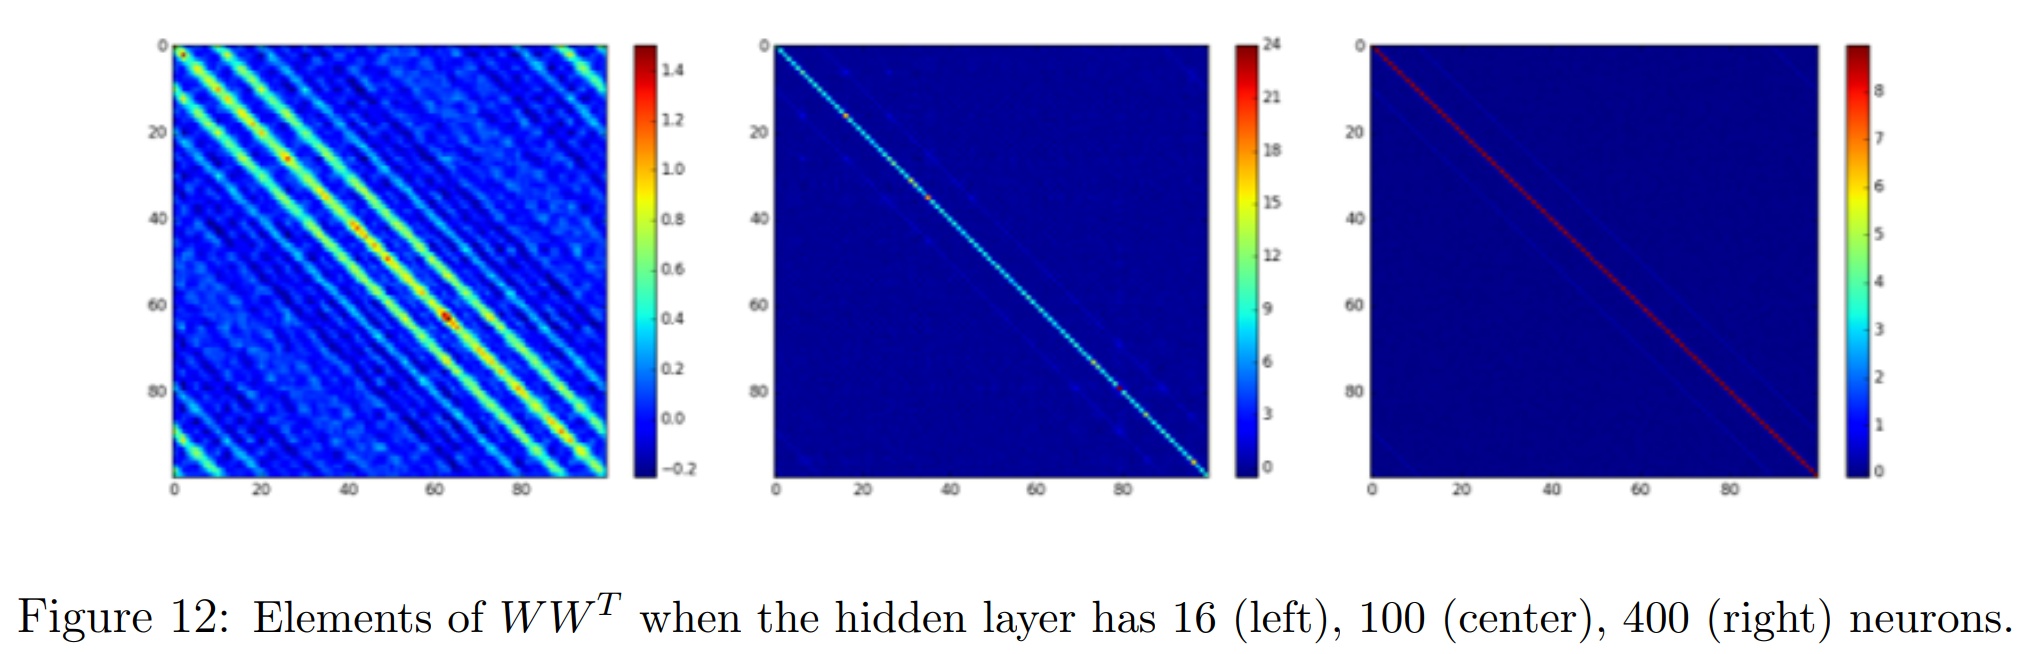
\includegraphics[height=3.6cm]{image/Figure12.png}
    \end{center}
  \end{figure}
  \underline{図からわかること}
  \vspace{0.2cm}
  \begin{itemize}
    \item どの場合も対角成分の値は大きい
    \item $N_h=400$,$N_h=100$の時は対角行列に近い
    \item $N_h=16 < 100$の時,非対角成分にも大きな値が存在
  \end{itemize}
  \vspace{0.3cm}
  $\Rightarrow$ \ $N_h=16$の時の$WW^{\top}$は入力配位のスピン相関を反映しているに違いない!!
\end{frame}

\begin{frame}{4.2 \ $WW^{\top}$におけるスピン相関}
  \begin{columns}
     \begin{column}{0.4\textwidth}
      \underline{図からわかること}
      \vspace{0.2cm}
      \begin{itemize}
        \item $WW^{\top}$の相関は高温でより急速に減少\\
        $\Rightarrow$RBMは相関距離(クラスターのサイズ)を正確に学習している
        \vspace{0.5cm}
        \item TypeVはT=2とT=3の間\\
        $\Rightarrow$TypeVのRBMは$T_c$付近の配位と似た特徴を取得した
      \end{itemize}
     \end{column}
     \begin{column}{0.6\textwidth}
      \begin{figure}
        \begin{center}
          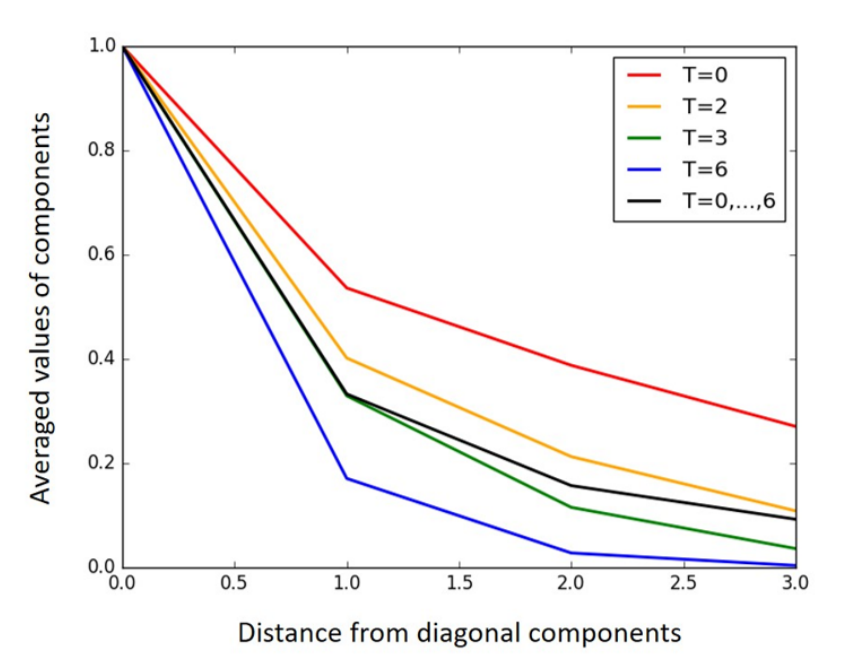
\includegraphics[height=4.6cm]{image/Figure13.png}
        \end{center}
      \end{figure}
     \end{column}
  \end{columns}
\end{frame}

\section{4.3 \ 磁化と特異値分解(SVD)}
\begin{frame}[t]{4.3 \ 磁化と特異値分解(SVD)}
  $WW^{\top}$の固有値,固有ベクトルをそれぞれ$\lambda_a , u_a \ (a=1,\dots,N_h)$とする
  \begin{equation*}
    WW^{\top}u_a = \lambda_a u_a
  \end{equation*}
  入力の配位ベクトル$v^{(0)}$は固有値ベクトルを使って$v^{(0)}=\sum_{a}c_a u_a \ $(規格化条件: $\sum_{a}(c_a)^2$=1)のように分解することができるので
  \begin{align*}
    v^{(0)\top}WW^{\top}v^{(0)\top}
    &= \left(\sum_a c_a u_a\right)^{\top}WW^{\top}\left(\sum_a c_a u_a\right)\\
    &= \left(\sum_a c_a u_a\right)^{\top}\left(\sum_a c_a \lambda_a u_a\right)\\
    &= \sum_a \sum_{a'} c_a c_{a'} \lambda_{a'} (u_a)^{\top}u_{a'}\\
    &= \sum_a c_a^2 \lambda_a
  \end{align*}
  $\Rightarrow$ $v^{(0)}$が$WW^{\top}$の固有値の要素を多く含んでいれば$v^{(0)\top}WW^{\top}v^{(0)\top}$の値が大きくなる
\end{frame}

\begin{frame}[t]{4.3 \ 磁化と特異値分解(SVD)}
  \begin{figure}
    \begin{center}
      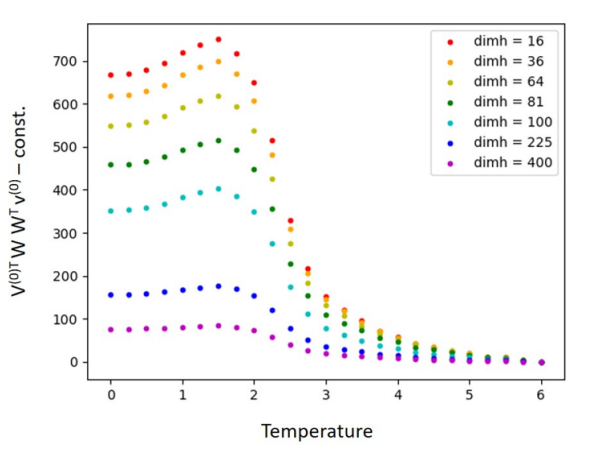
\includegraphics[height=6cm]{image/Figure14.png}
    \end{center}
  \end{figure}
  \begin{itemize}
    \item 臨界点付近で大きな変化(イジングモデルの磁化を思わせる)
  \end{itemize}
\end{frame}

\begin{frame}[t]{4.3 \ 磁化と特異値分解(SVD)}
  \begin{columns}
    \begin{column}{0.5\textwidth}
      \begin{figure}
        \begin{center}
          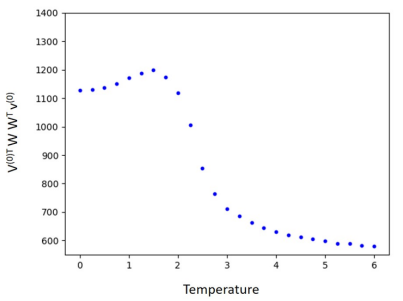
\includegraphics[height=3.8cm]{image/Figure15_left.png}
        \end{center}
      \end{figure}
      \begin{figure}
        \begin{center}
          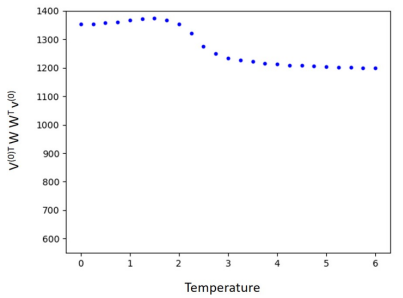
\includegraphics[height=3.8cm]{image/Figure15_right.png}
        \end{center}
      \end{figure}
    \end{column}
    \begin{column}{0.5\textwidth}
      \begin{figure}
        \begin{center}
          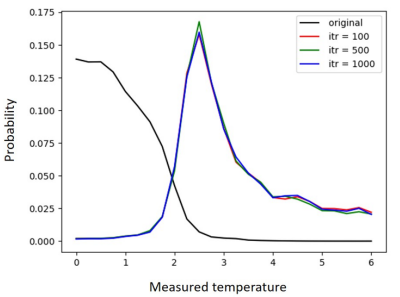
\includegraphics[height=3.7cm]{image/Figure6_right.png}
        \end{center}
      \end{figure}
      \begin{figure}
        \begin{center}
          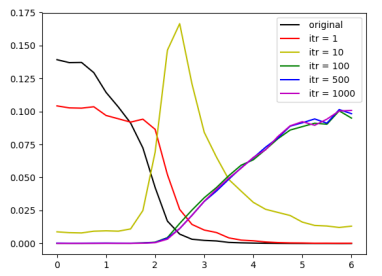
\includegraphics[height=3.5cm]{image/Figure9.png}
        \end{center}
      \end{figure}
    \end{column}
  \end{columns}
\end{frame}

\begin{frame}[t]{4.3 \ 磁化と特異値分解(SVD)}
  \underline{図15から分かること}
  \vspace{0.2cm}
  \begin{itemize}
    \item $N_h$が大きい時と小さいと時で臨界点付近での値の変化量が異なる\\
    \vspace{0.2cm}
    $\rightarrow$この違いが図6と図9のRBMフローの違いを引き起こす原因?
    \item $H_h$が大きいときは高温の時も値が大きい\\
    \vspace{0.2cm}
    $\rightarrow$$N_h$が大きいRBMは高温における特徴をより多く学習しているのではないか?
  \end{itemize}
  \vspace{0.2cm}
  これは第3.2節の2番目の予想に他ならず,これは,4.2章のスピン相関の振舞いで裏付けられている!!!
\end{frame}

\section{4.4 \ 固有値スペクトルとWに格納された情報}
\begin{frame}[t]{4.4 \ 固有値スペクトルとWに格納された情報}
  \begin{figure}
     \begin{center}
         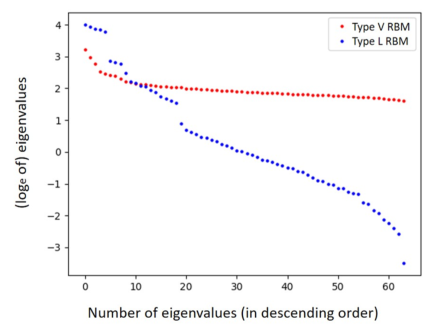
\includegraphics[height=3.5cm]{image/Figure16.png}
     \end{center}
  \end{figure}
  \underline{図16からわかること}
  \vspace{0.2cm}
  \begin{itemize}
    \item Type Lではいくつかの固有値だけが値が大きい\\
    \vspace{0.2cm}
    $\Rightarrow$ Type L RBMは,隠れ層のニューロンは少数で十分
    \item Type Vでは固有値の値は緩やかに減少\\
    \vspace{0.2cm}
    $\Rightarrow$ Type V RBMは,すべての固有ベクトルが均等に利用されている
  \end{itemize}
  \vspace{0.2cm}
  $\Rightarrow$広い温度範囲の特徴を学習するには,隠れ層に多くのニューロンが必要!!
\end{frame}

\begin{frame}[t]{4.4 \ 固有値スペクトルとWに格納された情報}
  \begin{figure}
     \begin{center}
         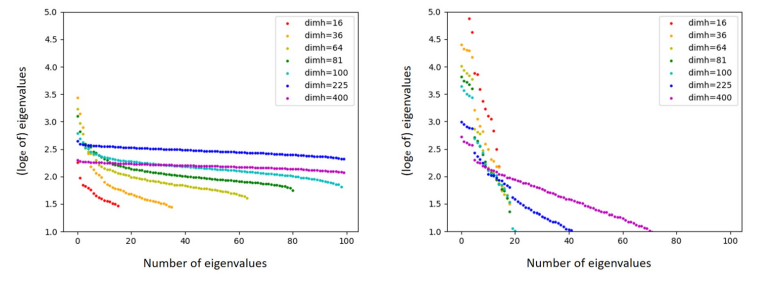
\includegraphics[height=4cm]{image/Figure17.png}
     \end{center}
  \end{figure}
\end{frame}

\end{document}